
\documentclass[twoside]{article}
\usepackage{CJKutf8}

%\usepackage{graphics}
\usepackage{graphics}
\usepackage{geometry}
\usepackage{forest,amsmath}
\usepackage{enumerate}
\usepackage{url}
\usepackage{latexsym,bm,amssymb}

\geometry{left=2.5cm,right=2cm,top=2.5cm,bottom=2.5cm}

%\setlength{\oddsidemargin}{0.25 in}
%\setlength{\evensidemargin}{-0.25 in}
%\setlength{\topmargin}{-0.6 in}
%\setlength{\textwidth}{6.5 in}
%\setlength{\textheight}{8.5 in}
%\setlength{\headsep}{0.75 in}
\setlength{\parindent}{0 in}
\setlength{\parskip}{0.1 in}

\usepackage{listings}
\usepackage{color}
\renewcommand\lstlistingname{Quelltext} % Change language of section name
\lstset{ % General setup for the package
    language= C,
    %basicstyle=\small\sffamily,
    basicstyle=\ttfamily,
    numbers=left,
     numberstyle=\tiny,
    frame=tb,
    tabsize=4,
    columns=fixed,
    showstringspaces=false,
    showtabs=false,
    keepspaces,
    commentstyle=\color{red},
    keywordstyle=\color{blue}
}

%
% The following commands set up the lecnum (lecture number)
% counter and make various numbering schemes work relative
% to the lecture number.
%
%\newcounter{lecnum}
%\renewcommand{\thepage}{\thelecnum-\arabic{page}}
%\renewcommand{\thesection}{\thelecnum.\arabic{section}}
%\renewcommand{\theequation}{\thelecnum.\arabic{equation}}
%\renewcommand{\thefigure}{\thelecnum.\arabic{figure}}
%\renewcommand{\thetable}{\thelecnum.\arabic{table}}

%
% The following macro is used to generate the header.
%


%


%Use this command for a figure; it puts a figure in wherever you want it.
%usage: 
%\begin{figure}
%\begin{center}
%\includegraphics[width=5in]{fig-file}
%\caption{}\label{fig:delavl}
%\end{center}
%\end{figure}

%%% Use the following command for a table
%%%

% Use these for theorems, lemmas, proofs, etc.
\newtheorem{theorem}{Theorem}[theorem]
\newtheorem{lemma}[theorem]{Lemma}
\newtheorem{proposition}[theorem]{Proposition}
\newtheorem{claim}[theorem]{Claim}
\newtheorem{corollary}[theorem]{Corollary}
\newtheorem{definition}[theorem]{Definition}
\newenvironment{proof}{{\bf Proof:}}{\hfill\rule{2mm}{2mm}}

% **** IF YOU WANT TO DEFINE ADDITIONAL MACROS FOR YOURSELF, PUT THEM HERE:

\begin{document}
\begin{CJK*}{UTF8}{gbsn}
	%FILL IN THE RIGHT INFO.
	%\lecture{**LECTURE-NUMBER**}{**DATE**}{**LECTURER**}{**SCRIBE**}
	%\lecture{1}{Project Name}{Deshi Ye}{Student 1, Student 2, 学生3}
	%\footnotetext{These notes are partially based on those of Nigel Mansell.}
	\title{Flexible}
	\date{}
	%\maketitle
	% **** YOUR NOTES GO HERE:

	% Some general latex examples and examples making use of the
	% macros follow.  
	%**** IN GENERAL, BE BRIEF. LONG SCRIBE NOTES, NO MATTER HOW WELL WRITTEN,
	%**** ARE NEVER READ BY ANYBODY.
	\section{Introduction}
	After printing many review materials double-sided, we find it disturbing to flip them upside down during the review. Assume that N pages of the materials are double-sided printed, each side containing one of N chapters in the textbook. We wonder if there is a way to flip some of them so that we can cover all the N chapters at once.
	
	In this program, we need to find out one flipping solution, which can let us cover all the N chapters at once.
	
	For example if the Input is following :
	
	5\\
	3 2 \\2 5 \\4 1 \\1 3 \\2 1\\
	
	The output should be :
	3 5 4 1 2
	(ignore the echo of input)
	
	That means if we just flip the second page (swap 2 5 , the third line of input), and then we will get the first colum as the answer, which let us cover all the 5 chapters at once.
	
	
	\section{Algorithm Specification}
	
	The first thing we should do is read the input and do process of them. We use \textbf{trap x20} to read. Because the $N$ may be larger than $10$, we should use the special character like \textbf{Space} and \textbf{Enter} as a signal. After finishing the read of a number ,we transfer it into digit rather than ascii code and store it into memory.
	
	\begin{lstlisting}[mathescape=true]
		num $\leftarrow$ 0 \\ initialize
		trap x20
		trap x21
		while R0 != \n
			num $\leftarrow$ 10 * num + R0 - '0'
		for i = 0 to num-1
			num $\leftarrow$ 0 \\ initialize
			trap x20
			trap x21
			while R0 != ' '
				num $\leftarrow$ 10 * num + R0 - '0'
			page[2*i] $\leftarrow$ num
			num $\leftarrow$ 0 \\ initialize
			trap x20
			trap x21
			while R0 != ' '
				num $\leftarrow$ 10 * num + R0 - '0'
			page[2*i + 1] $\leftarrow$ num			
	\end{lstlisting}
	 
	Then, we use the recursion to determine the flip condition. To simplify the coding procedure, we use an array to store whether one page need flip.
	Once we determine the ith page need to flip, then we recursively call function itself to get the flip condition of (i+1)th page to nth page. This procedure will form a complete binary tree. When the program comes to the leave of the binary tree, the program will call the check function to check whether in this flip condition, we can cover all the N chapters at once.
	
	\begin{lstlisting}[mathescape=true]
	function flip(int n) 
		if n == num
			call check()
			return
		flip[n] $\leftarrow$ 0
		call flip(n-1)
		flip[n] $\leftarrow$ 1
		call flip(n-1)
		flip[n] $\leftarrow$ 0 \\recover to be init
	\end{lstlisting}

	

	When the program comes to the leave of binary tree, the check function will be called. In the check function, we check whether the chosen chapter of each page can cover from 1 to num. Firstly, according to the flip condition, we take out the front chapter or back chapter of each page and store the result into memory. Then we form a label area, according to the result we get before to set the label area. That means if the result contain chapter 4, then label[3] will be set to 1. Finally, we go through the label area. If it's all 1 in label area, then we just output the result we obtained before and halt the program.
	
	\begin{lstlisting}[mathescape=true]
	function check() 
		for i = 0 to num - 1
			if flip[i] == 1
				result[i] $\leftarrow$ page[2*i + 1]
			else 
				result[i] $\leftarrow$ page[2*i]
		// clear the label area
		for i = 0 to num - 1
			label[i] $\leftarrow$ 0
		for i = 0 to num - 1
			label[result[i]-1] $\leftarrow$ 1
		for i = 0 to num - 1
			if label[i] == 0
				return
		//output
		for i = 0 to num - 1
			R0 $\leftarrow$ result[i]
			trap x21
		halt
	\end{lstlisting}

	\section{Q and A}
	\begin{itemize}
		\item 	Q: what is your recursive algorithm?
		
				A: in the program, we do the recursive algorithm accroding to the flip condition. Once we set the ith page to be flipped or not, we then recursively set the (i+1)th to nth pages. In this way, the program will form a binary tree. When the program comes to the leave of binary tree, we call the check function to check the condition.
	\end{itemize}


	\section{essential parts of code}
	Fig 1 is the implement of recursion operation
	\begin{figure}[htbp]
		\small
		\centering
		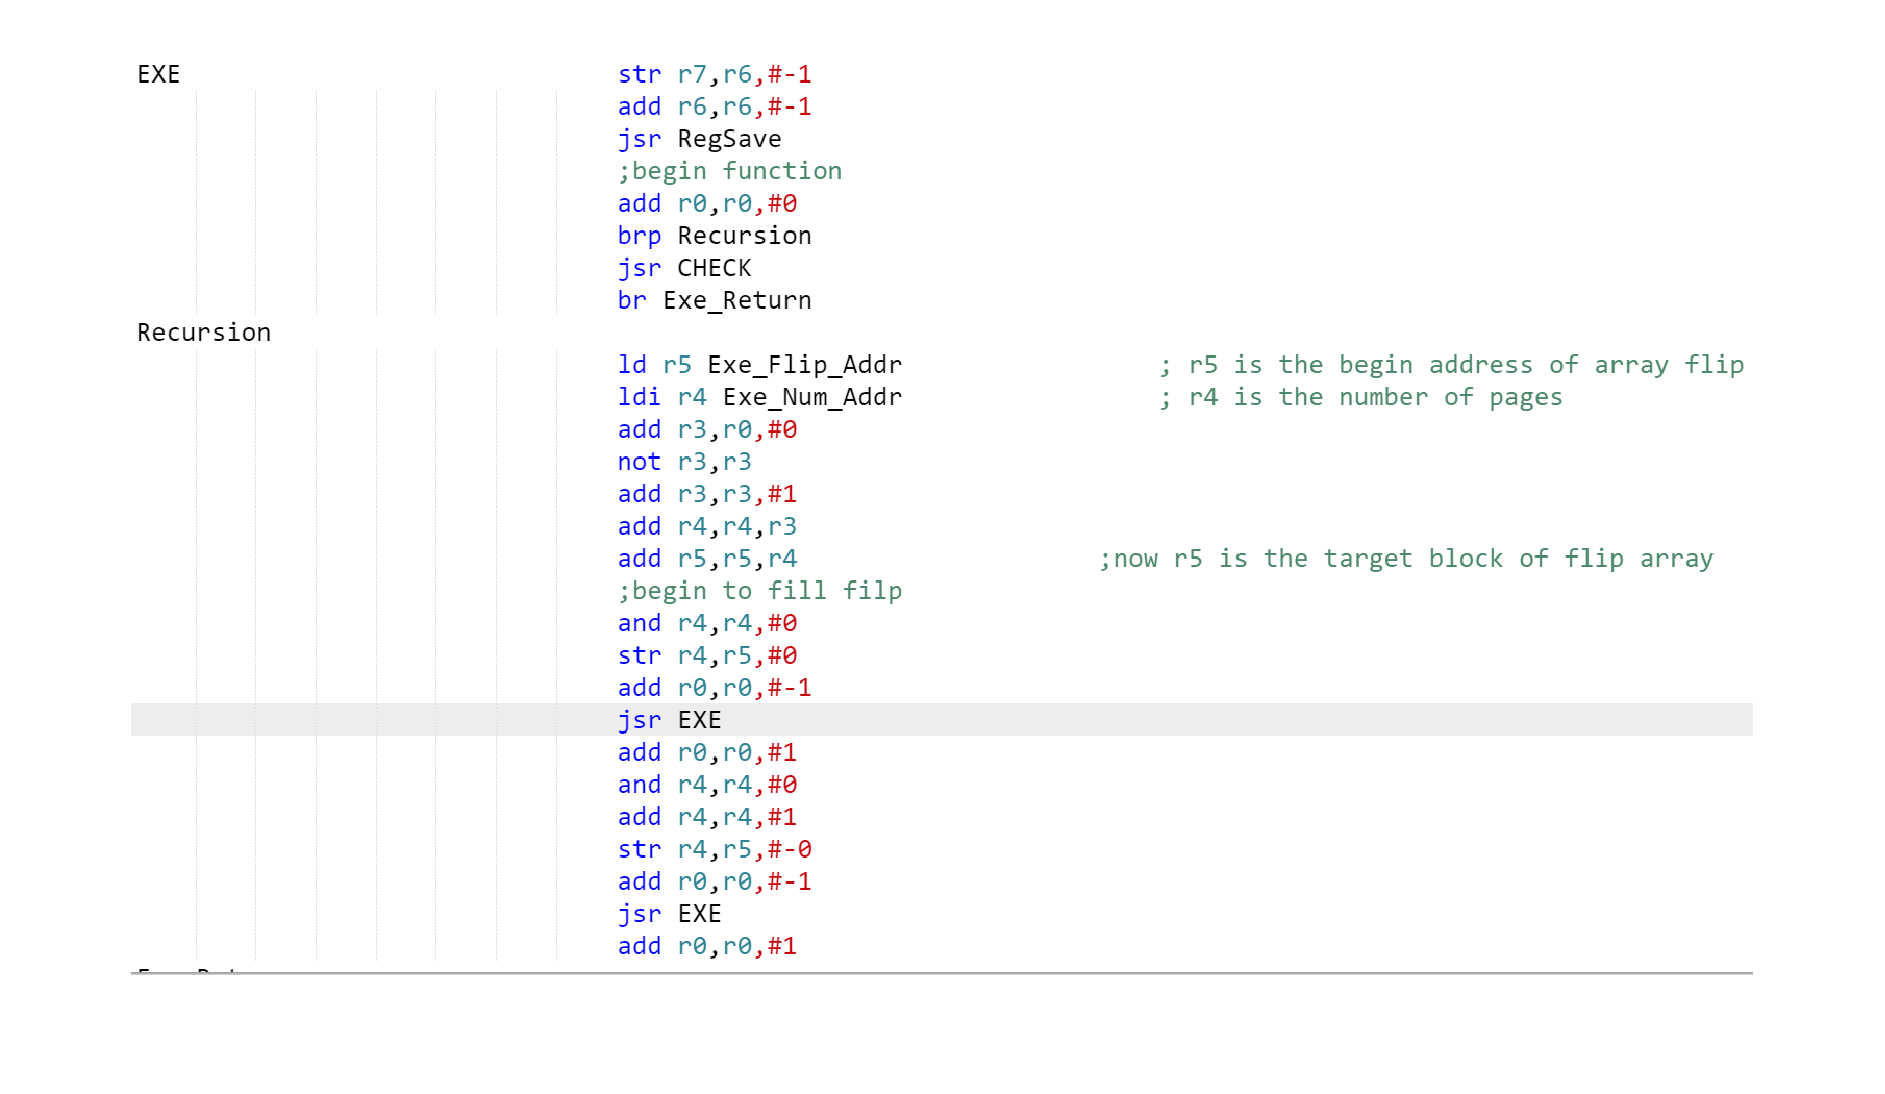
\includegraphics[width=0.7\textwidth]{2.eps}
		\caption{Fig 1} %名字
	\end{figure}
	
	
	Fig 2 is the implement of check function

	\begin{figure}[htbp]
		\centering
		\caption{Fig 2} %名字
		\begin{minipage}[t]{0.4\textwidth}
			\small
			\centering
			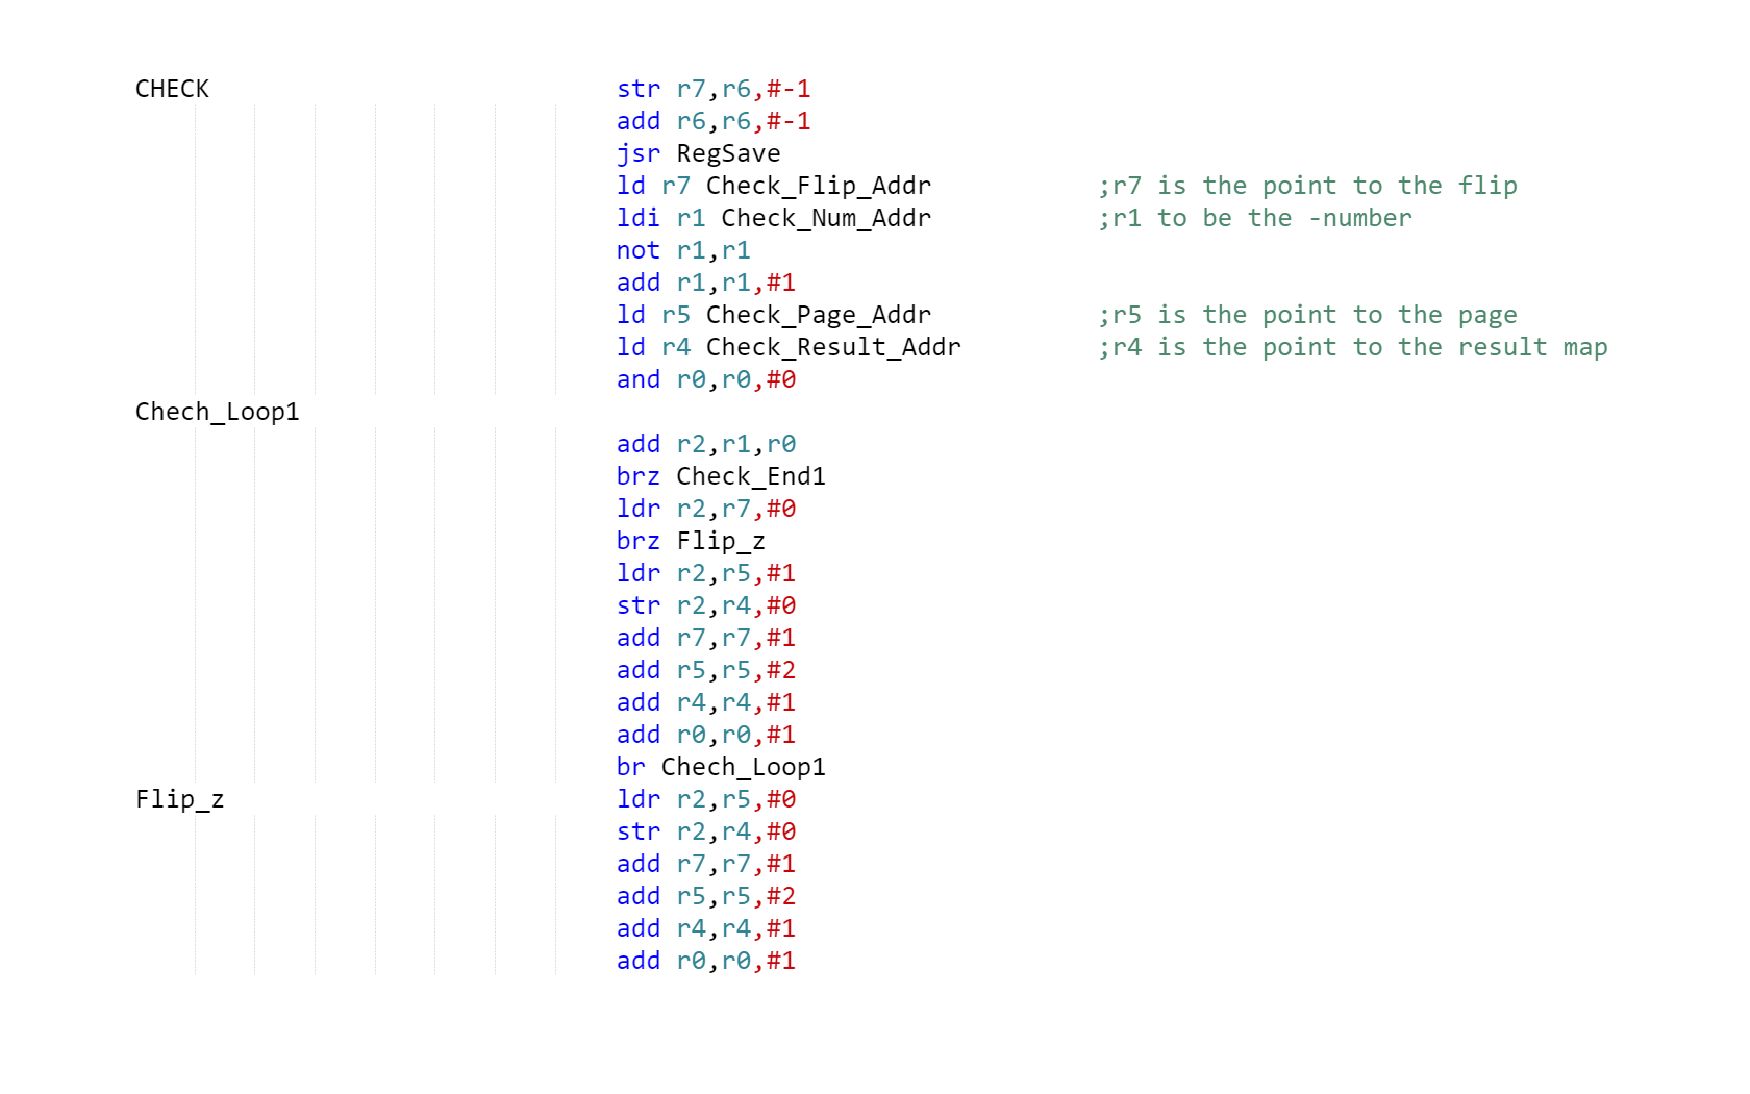
\includegraphics[width=0.9\textwidth]{3.eps}
		\end{minipage}
		\begin{minipage}[t]{0.4\textwidth}
			\small
			\centering
			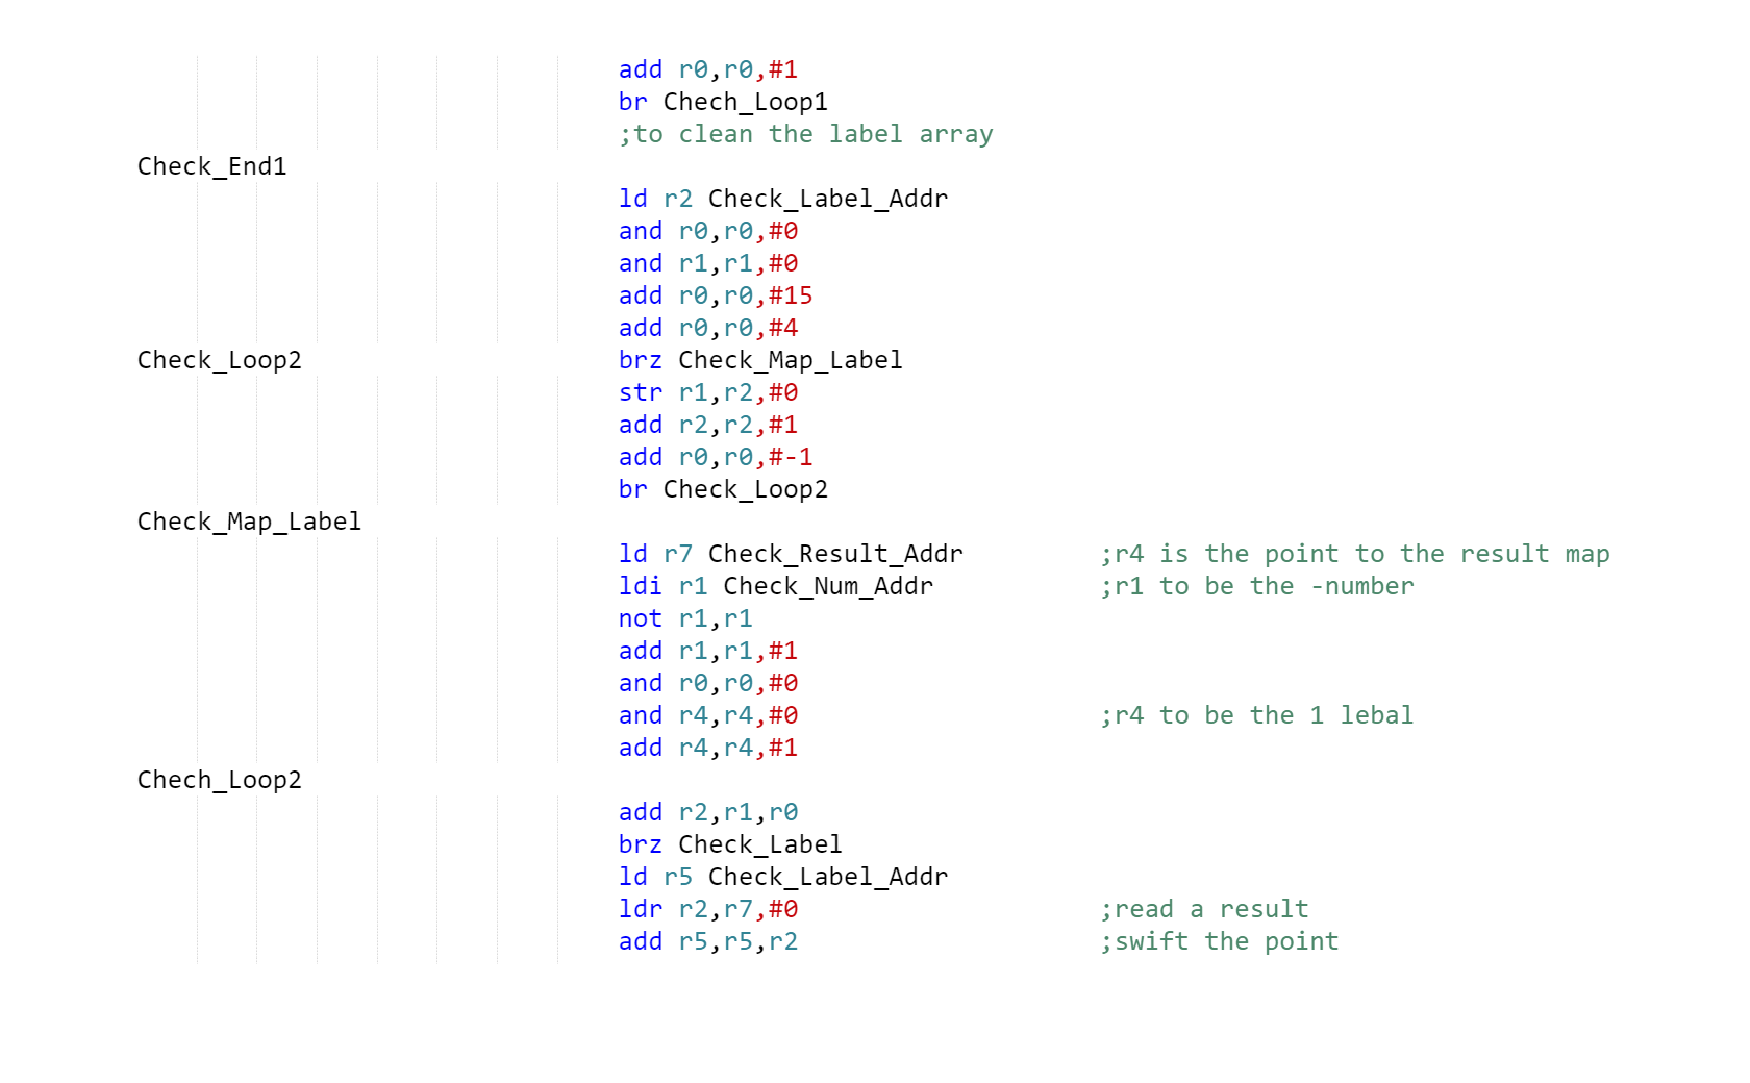
\includegraphics[width=0.9\textwidth]{4.eps}
		\end{minipage}
		\begin{minipage}[t]{0.4\textwidth}
			\small
			\centering
			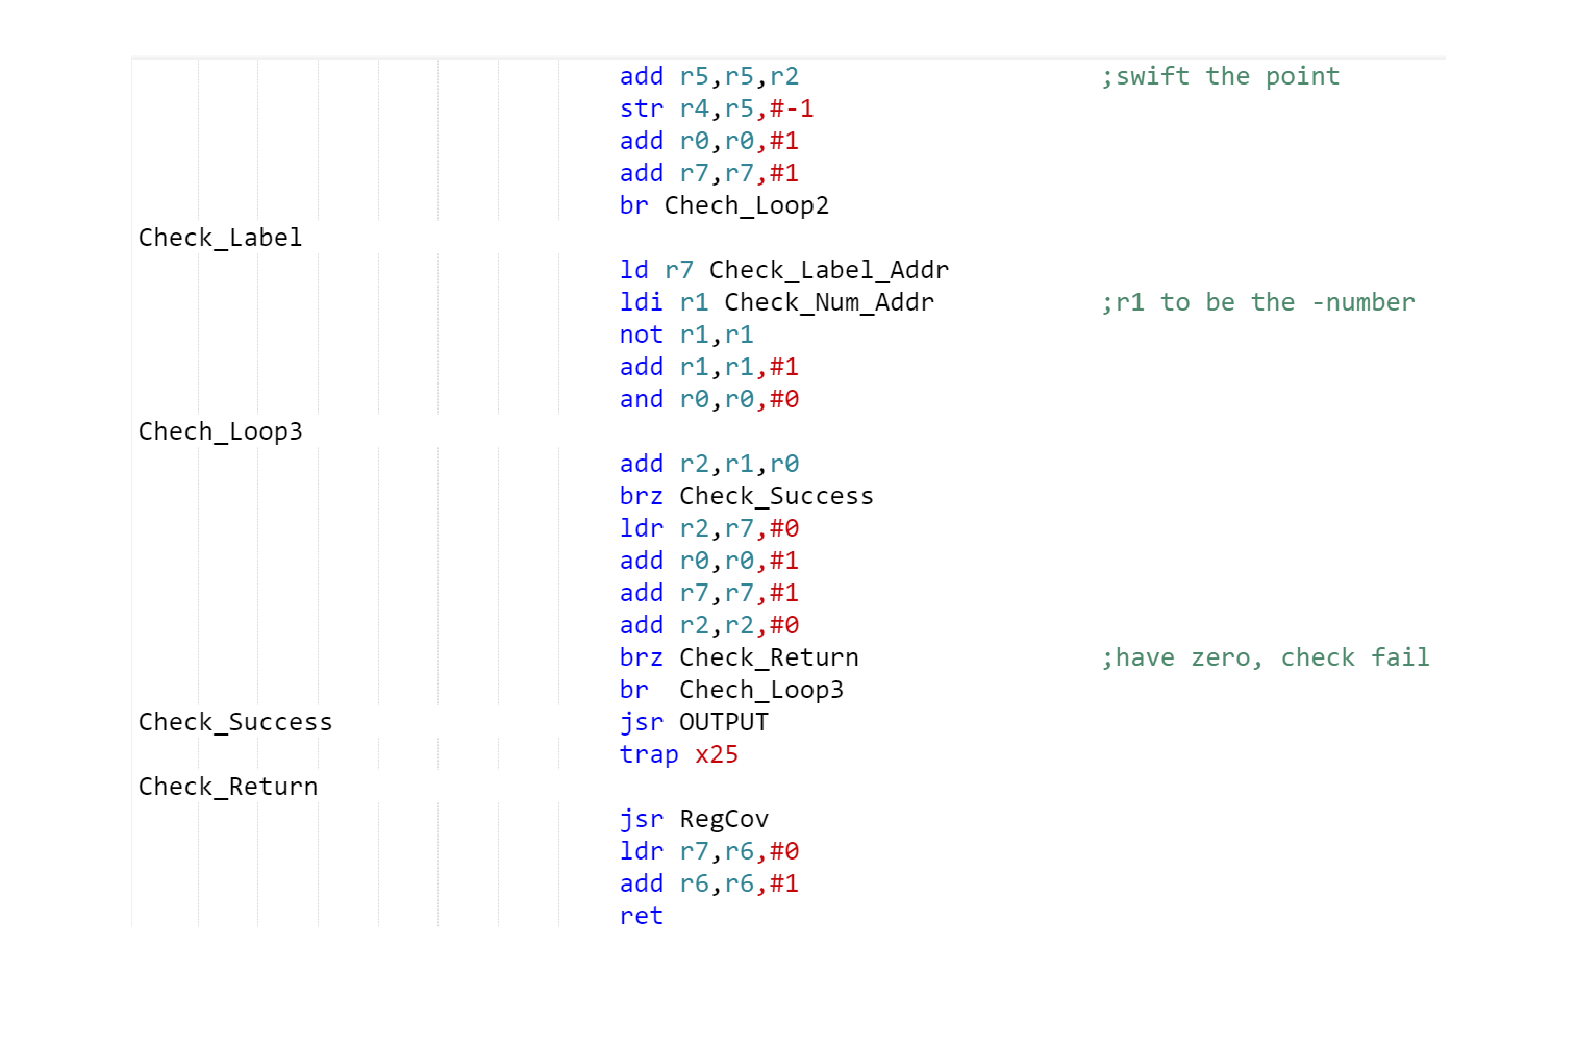
\includegraphics[width=0.9\textwidth]{1.eps}
		\end{minipage}
		
	\end{figure}


\end{CJK*}
\end{document}





